\chapter{Color-Ordered Feynman Rules}
\label{sec:cofr}

For completeness, we provide the QCD color-ordered Feynman rules,
which are used for the computation of  color-ordered amplitudes.
All external legs are cyclically-ordered, and all external momenta are outgoing.
The derivation can be found e.g.\ in \cite{Mangano1991}.
We do not provide the Feynman rules for ghosts, since we do not need to consider their contributions in out computations.

A nice summary tables of the complete set of SM Feynman rules can be found in\cite{Romao:2012pq}.


\begin{table}[]
\centering
\caption{Color-ordered QCD Feynman rules }
\label{tab:frqcd}
\begin{tabular}{l}
\begin{tabularx}{\textwidth}{ll}
    \hline
    \noalign{\vskip 4mm}
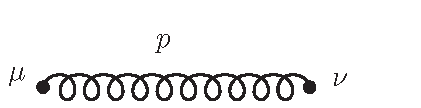
\includegraphics[clip,width=0.2\textwidth]{figures/gp2}
&$\displaystyle ~ \frac{-ig^{\mu\nu}}{p^2}$ \qquad {\footnotesize (Feynman gauge)}\\
    \noalign{\vskip 2mm}
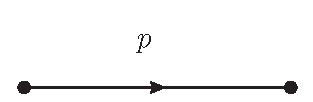
\includegraphics[clip,width=0.15\textwidth]{figures/qp2} &
$\displaystyle  ~ \frac{i(\slashed{p}+m)}{p^2-m^2}$\\
    \noalign{\vskip 4mm}
\raisebox{-.4\height}{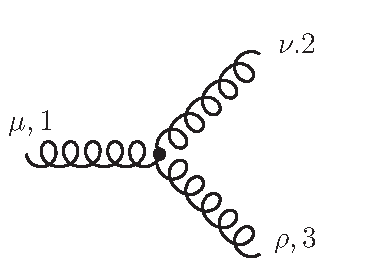
\includegraphics[clip,width=0.2\textwidth]{figures/gggv}}
& $\displaystyle ~ \frac{i}{\sqrt{2}} \left[
        g^{\mu\nu}(p_1-p_2)^\rho+g^{\nu\rho}(p_2-p_3)^\mu+g^{\rho\mu}(p_3-p_1)^\nu\right]$\\
\raisebox{-.4\height}{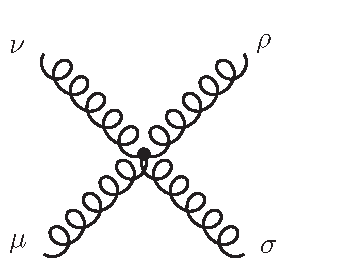
\includegraphics[clip,width=0.2\textwidth]{figures/gggg}}
&  $\displaystyle~ i \left[ g^{\mu\rho}g^{\nu
        \sigma}-\frac{1}{2}(g^{\mu\nu}g^{\rho\sigma}+g^{\mu\sigma}g^{\nu\rho})\right]$ 
\end{tabularx}\\
    \noalign{\vskip 2mm}
\begin{tabularx}{\textwidth}{lp{4.5cm}ll}
\raisebox{-.4\height}{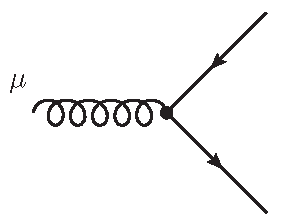
\includegraphics[clip,width=0.15\textwidth]{figures/qqg}}
&
$\displaystyle~ \frac{i}{\sqrt{2}} g_{s} \gamma^{\mu}$&
\raisebox{-.4\height}{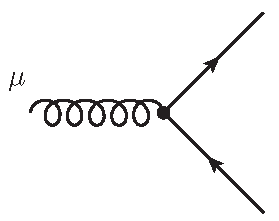
\includegraphics[clip,width=0.15\textwidth]{figures/qqg2}}
&
 $ \displaystyle~  -\frac{i}{\sqrt{2}} g_{s} \gamma^{\mu}$\\
\end{tabularx}\\

\end{tabular}
\end{table}





%\chapter{Results for Selected Scalar Integrals}
%\label{sec:massivebasisint}
%Among the additional scalar integrals appearing in the master
%integral decomposition in Section \ref{sec:scmi} for processes involving massive quarks are the
%tadpole integral $I_1(m^2)$ and the bubble integral with a single massive leg in
%one corner $I_2(m^2;0,m^2)$. For vanishing masses, both
%integrals are scaleless and vanish in dimensional regularization. They
%are given in dimensional regularization with $D=4-2\epsilon$ by
%\begin{align}\label{eq:tadint}
%I_1(m^2) \coloneqq I_{1}=\frac{\mu_R^{2\epsilon}}{ic_{\Gamma}}\int
  %\frac{\dd[D]{\ell}}{(2\pi)^D}\frac{1}{(\ell^2-m^2)} =
   %m^2\left(\frac{1}{\epsilon}+\log(\frac{\mu_R^2}{m^2})+1 \right)+\mathcal{O}(\epsilon),
%\end{align}
%and
%\begin{align}\label{eq:olbmint}
%I_2(m^2;0,m^2) \coloneqq
%I_{2,m^2}=\frac{\mu_R^{2\epsilon}}{ic_{\Gamma}} \int
  %\frac{\dd[D]{\ell}}{(2\pi)^D}\frac{1}{\ell^2((\ell-p)^2-m^2)} =
  %\left(\frac{1}{\epsilon}+\log(\frac{\mu_R^2}{m^2})+2 \right)+\mathcal{O}(\epsilon),
%\end{align}
%where the small imaginary part $i\epsilon$ in the inverse propagators
%is understood implicitly as $D_i=(\ell_i^2-m_i^2+i\epsilon)$ and $c_\Gamma=(4\pi)^{-(2-\epsilon)}\Gamma^2(1-\epsilon)\Gamma(1+\epsilon)/\Gamma(1-2\epsilon)$. The integrals are taken from Ref.~\cite{Ellis:2007qk}.





%\chapter{Tadpole Coefficients From UV matching}
%\label{sec:uvmatch}
%In an application of numerical unitarity to processes with a single mass circulating in
%the loop, one can avoid the computation of single cuts in order to extract the
%tadpole coefficient.\footnote{For more complex processes with different masses
%in the loop one has several tadpole coefficients.} Instead, as
%proposed in Ref.~\cite{Bern:1995db,Badger2008}, one can match the known $UV$
%singularity structure of the mass-renormalized amplitude \cite{Catani:2000ef} to the $UV$ poles of tadpole, bubble and renormalization contributions. The
%$UV$-divergent part of the tadpole integral and bubble integrals are
%given in Eq.~\eqref{eq:tadint} and Eq.~\eqref{eq:olbmint} of Appendix \ref{sec:massivebasisint} by
%\begin{align}
 %I_{1\rvert_{\frac{1}{\epsilon}}} &= \tilde{I}_1 = m^2 &
 %I_{2,i\rvert_{\frac{1}{\epsilon}}} &= \tilde{I}_{2,i} = 1  
%\end{align}
%for all $i$ and are in particular independent of other kinematical
%invariants. Since tadpole and bubble integrals as well as mass renormalization counterterms are the only sources of $UV$ divergencies for
%mass-renormalized one-loop
%amplitudes, one can deduce the tadpole coefficient by matching the known
%$UV$-pole structure of each primitive amplitude \cite{Catani:2000ef} to the $UV$-poles of the
%combined bubble, tadpole and renormalization contributions
%\begin{align}
  %\begin{split}
  %\mathcal{A}_{\rvert_\text{UV}}^{\text{mass ren.}} & =  \sum_i b^0_i
  %\tilde{I}_{2,i}+a^0 \tilde{I}_1 + \alpha_{\text{mass ren.}}\\
%&\Rightarrow   a^0 =  \frac{1}{m^2}\left(\mathcal{A}_{\rvert_\text{UV}}^{\text{mass ren.}} -  \sum_i
%b^0_i  -\alpha_{\text{mass ren.}}\right) ,
  %\end{split}
%\end{align}
%with the mass renormalization contribution $\alpha_{\text{mass ren.}}$. In practice, this implies extracting the $UV$ pole structure
%of primitive amplitudes from that of the full amplitude
%\cite{Catani:2000ef} as laid
%out in Ref.~\cite{Ellis:2011cr}. In the work presented in this thesis we do
%not apply this technique but follow the straightforward application of numerical unitarity
%and compute single cuts explicitely. In particular since this is
%independent of the number of masses in the loop.






\chapter{The van Neerven-Vermaseren Basis}
\label{sec:vNV_basis}

The van Neerven-Vermaseren basis \cite{Neerven1984a,Ellis:2007br}
takes a list of $n<D$ vectors $\{p_1,\ldots{}p_n\}$ as an input, 
and decomposes the full vector space in $D$ dimensions $\mathsf{S}_{[D]}$ into
a direct sum,
\begin{subequations}
  \begin{gather}
    \mathsf{S}_{[D]} = \spn{v_1,\ldots{},v_n} \oplus \spn{\tau_1,\ldots{},\tau_{D-n}},
    \intertext{with $\spn{p_1,\ldots{},p_n} = \spn{v_1,\ldots{},v_n}$, and dual vectors $v_i = \qty(G^{-1})_{ij}\,p_j$, such that}
    \sp(\tau_i,p_j) = \sp(\tau_i,v_j) = 0, \\
    \sp(v_i,p_j) = \delta_{ij}, \qquad \sp(\tau_i,\tau_j) = \delta_{ij} (\tau_{j})^2,
  \end{gather}
\end{subequations}
where $G^{-1}$ is the inverse of the Gram matrix $G_{ij}=\sp(p_i,p_j)$.
The basis vectors of the transverse space $\tau_i$ can be obtained by projecting any $(D-n)$ linear independent seed vectors
into the transverse space with
\begin{align}\label{eq:metricpron}
  g_\tau^{\mu\nu} =  g^{\mu\nu} - \sum_{i=1}^{n}p_i^\mu v_i^\nu,
\end{align}
and orthogonalizing them via the Gram-Schmidt process.

The algorithm works for any dimension $D$ and metric signature.%
\footnote{There are some subtleties connected to non-positive-definite metric signatures (see e.g.\ the bubble topology in \cref{sec:ms_examples})}
It also works over arbitrary field as long as we don't require the transverse vectors to be normalized.


\chapter{Spinor-Helicity}
\label{chap:4dspinhel}

The spinor-helicity methods are well known are covered 
in great detail in numerous sources \todo{references}.
We provide only a brief summary.

Helicity of a particle is the projection of it's spin $\va{S}$ on the direction of it's
three-momentum $\va{p}$, and the states $\psi_{\pm s}$ with helicity $\pm s$ are defined as
\begin{equation} \label{eq:helicity_def}
  \sp(\va{S},\va{p}) \, \psi_{\pm s} = \pm s \abs{\va{p}}\, \psi_{\pm s}.
\end{equation}
The helicity of massless particles is a Lorentz invariant, and for spinor representations helicity and chirality eigenstates
coincide. 
%In fact the helicity eigenstates of massless particles are induced unitary representations
For massive particles helicity eigenstates can be constructed relative to a chosen reference frame.


\subsubsection{Massless Spin $1/2$}

For massless spin $\frac{1}{2}$ particles $\va{S} = \frac{1}{2}\va{\sigma}$, and 
the \cref{eq:helicity_def} is written in a covariant way as
\begin{equation}
  (\sp(p,\bar{\sigma}))^{\dot{A}B} \lambda_B(p) = 0, \qquad (\sp(p,\sigma))_{A\dot{B}} \lambda^{\dot{B}}(p) = 0,
\end{equation}
for positive and negative helicities correspondingly.
Here 
\begin{equation}
  \sigma_{A \dot{B}}^{\mu} \coloneqq  \left( 1 , - \vec{\sigma} \right) \qand \bar{\sigma}^{\mu \dot{A} B} \coloneqq  \left( 1 ,  \vec{\sigma} \right),
  \qquad \vec{\sigma}\coloneqq (\sigma_x,\sigma_y,\sigma_z),
\end{equation} 
with the standard Pauli matrices
\begin{eqnarray}
  \sigma_x = \left(\begin{array}{cc}
    0 & 1\\
    1 & 0 \\
  \end{array} \right),
  &
  \sigma_y = \left(\begin{array}{cc}
    0 & -i\\
    i & 0 \\
  \end{array} \right),
  &
  \sigma_z = \left(\begin{array}{cc}
    1 & 0\\
    0 & -1 \\
  \end{array} \right),
\end{eqnarray}
and we introduced dotted and undotted spinor indices corresponding to the two non-equivalent representation of $SL(2,\mathbb{C})$.
The indices can raised and lowered with the 2-dimensional Levi-Civita symbol as
\begin{equation}
    \label{raising_and_lowering_spinor_indices}
  \begin{gathered}
    p^A = \varepsilon^{AB} p_B, \qquad
    p^{\dot{A}} = \varepsilon^{\dot{A}\dot{B}} p_{\dot{B}}, \\
    p_{\dot{B}} = p^{\dot{A}} \varepsilon_{\dot{A}\dot{B}},  \qquad
    p_B = p^A \varepsilon_{AB},
  \end{gathered}
\end{equation}
which satisfies the properties
\begin{equation}
  \begin{gathered}
    \varepsilon_{BA} = - \varepsilon_{AB},  \quad   \varepsilon^{AB} = \varepsilon^{\dot{A}\dot{B}} = \varepsilon_{AB} = \varepsilon_{\dot{A}\dot{B}}, \\
    \eps^{A C} \eps_{B C} = \delta^{A}_{\;B}, \quad \eps^{\dot{A} \dot{C}} \eps_{\dot{B} \dot{C}} = \delta^{\dot{A}}_{\;\dot{B}}.
  \end{gathered}
\end{equation}
We will use a convenient notation of angle and square brackets,
\begin{equation}
  \begin{aligned}
    \ket{p} &\coloneqq \lambda_A(p), \quad \bra{p} &\coloneqq \lambda^A(p),  \\
    \sket{p} &\coloneqq \lambda^{\dot{A}}(p), \quad \sbra{p} &\coloneqq \lambda_{\dot{A}}(p),
  \end{aligned}
\end{equation}
to write compactly the spinor products,
\begin{subequations}
  \begin{equation}
    \spaa(p,q) \coloneqq \lambda^A(p) \lambda_A(q), \qquad \spbb(p,q) \coloneqq \lambda_{\dot{A}}(p) \lambda^{\dot{A}}(q),
  \end{equation}
  and spinor chains such as
  \begin{equation} \label{eq:vectors_from_spinors}
    \sbraket(p,\gamma^\mu,q) = \brasket(q,\gamma^\mu,p)  \coloneqq \lambda_{\dot{A}}(p) \bar\sigma^{\mu\dot{A}B} \lambda_B(q).
  \end{equation}
\end{subequations}

\todo{explicit form} 

\todo{denormalized spinors for finite fields}


\subsubsection{Massless Spin 1}

It is easy to see that the spinor chains of the form of \cref{eq:vectors_from_spinors} are mass Lorentz vectors, and
the helicity eigenstates of vector particles can be constructed as
\begin{equation}
  \varepsilon_+^\mu(p,\eta) = -\frac{\sbraket(p,\gamma^\mu,\eta)}{\sqrt{2} \spaa(p,\eta)}, \qquad \varepsilon_-^\mu(p,\eta) = \frac{\brasket(p,\gamma^\mu,\eta)}{\sqrt{2} \spbb(p,\eta)},
\end{equation}
where $\eta$ is some arbitrary reference vector. Indeed
the relations 
\begin{equation}
  \qty(\varepsilon_{\pm})^2 =0, \qquad
  \varepsilon^{\mu}_{\pm}(p,\eta) p_\mu = 0,
  \;\;\;\;
  \varepsilon^{\mu}_{\pm}(p,\eta) \eta_\mu = 0,
\end{equation}
are satisfied by construction, and the polarization sum is
\begin{equation}
  \varepsilon^{\mu}_{+}(p,\eta)\varepsilon^{\nu}_{-}(p,\eta) + \varepsilon^{\mu}_{-}(p,\eta)\varepsilon^{\nu}_{+}(p,\eta) = -g^{\mu\nu} + \frac{\ell^\mu \eta^\nu + \ell^\nu \eta^\mu}{\sp(\ell,\eta)}.
\end{equation}
And the little group scaling is
\begin{equation}
  \varepsilon_{\pm} \longrightarrow t^{(\mp 2)} \varepsilon_{\pm}
\end{equation}


\subsubsection{Massive Spin 1/2}


\todo{q-helicity little group}


\todo{Stefan's paper on spinors\cite{DittmaierWeyl}} 


\chapter{Clifford Algebras in $D_s$ Dimensions}
\label{sec:clifford_algebra_ds}

\todo{clean-up this significantly} 

\section{Representations}
The defining property of the Clifford algebra is
\begin{equation} \label{eqn:defClifford}
\acomm{\gamma_{[D_s]}^\mu}{\gamma_{[D_s]}^\nu} = 2 g_{[D_s]}^{\mu\nu}\mathbb{1}_{[D_s]}^{\vphantom{\mu\nu}},
\end{equation}
where $\mathbb{1}_{[D_s]}$ is the identity of the Clifford algebra.
The representations are constructed via recursive application of tensor products (see e.g.\ refs.~\cite{Collins:1984xc,Kreuzer:susylectures}):
\begin{align}\label{eq:gammait}
  \gamma^\mu_{[Ds]}  = 
  \begin{dcases}
    \mathbb{1}_{[2]} \otimes \gamma^\mu_{[D_s-2]}, & \mu =0\leq D_s-3,\\
    (\sigma_2\,\sigma_3) \otimes \gamma^\star_{[D_s-2]}, & \mu = D_s-2,\\
    (\sigma_3\,\sigma_1) \otimes \gamma^\star_{[D_s-2]}, & \mu = D_s-1,\\
  \end{dcases}
\end{align}
where $\{\sigma_1,\sigma_2,\sigma_3\}$ are Pauli matrices, and
\begin{equation}
  \begin{gathered}
    \gamma^\star_{[D_s]} \coloneqq i^{\frac{D_s}{2}-1} \gamma^0_{[D_s]}\cdots{}\gamma^{D_s -1 }_{[D_s]} ~\equiv~ \sigma_3 \otimes \gamma^\star_{[D_s-2]}, \\
    \acomm{\gamma^\star_{[D_s]}}{\gamma^\mu_{[D_s]}}=0, \qquad \gamma^\star_{[D_s]} \gamma^\star_{[D_s]} = \mathbb{1}_{[D_s]}.
  \end{gathered}
\end{equation}
We can thus write the Clifford algebra in $D_s$ dimensions in a factorized way,
\begin{equation}\label{eqn:cliffordrecursion}
  \qty(\gamma_{[D_s]}^\mu)_{a\kappa}^{\,b\lambda}  =
  \begin{dcases}
    \qty(\gamma_{[4]}^\mu)_a^{\;b} \, \delta_\kappa^\lambda\,, &  0\le\mu \le 3 \,,\\
    \qty(\gamma^{\star}_{[4]})_a^{\;b} \qty(\gamma_{[D_s-4]}^{(\mu-4)})_\kappa^{\;\lambda}\,, & \mu>3 \,,
  \end{dcases}
\end{equation}
where the indices $a,b$ denote the spinor indices in $\mathsf{S}_{[4]}$ and $\kappa,\lambda$ the ones in $\mathsf{S}_{[D_s - 4]}$.
Note that $\gamma^\mu_{[D_s-4]}$ represent a $(D_s-4)$-dimensional Clifford algebra.

%The spinor states for a particle with momentum $p$ satisfy the Dirac equation
%\begin{equation}
  %\qty(\slashed{p}_{[D_s]} \pm m \cdot \mathbb{1}_{[D_s]}) \psi  = 0,
%\end{equation}
\section{Basis}
\label{sec:identities}

In the following we derive the values of the contraction of the
tensors $w_0$ and $v_n$ which are used in 
eqs.~\eqref{eq:decompqqbar} and \eqref{eqn:4qampltensor}.
%
In this appendix we take $d$ to be an even integer denoting the
dimension of the space for which the Clifford algebra is defined
and we denote the dimension of the $\gamma$-matrix
representation by
$d_t=\Tr(\mathbb{1}_{[d]})=2^{d/2}$.
In the main text, we are interested in the case
%
\begin{eqnarray}
  d = (D_s-4)\,.
\end{eqnarray}
%
Since amplitude computations are homogeneous in the
factor $d_t$, it can be factored out and replaced by 
a suitable value in order to suit the four-dimensional 
limit. In this appendix, we keep the parameter $d_t$ in analytic
form in order to maintain a consistent finite-dimensional
algebra and for clarity of the equations. 
In the main text we use formulas with the replacement
$d_t\rightarrow 1$ imposed, which is the value consistent with a
calculation in dimensional regularization \cite{Collins:1984xc}.

We start with the trivial case of $w_0$ which appears in 
eq.~\eqref{eq:decompqqbar}. It is easy to find that
%
\begin{eqnarray}
  w_0=\delta_\kappa^\lambda\,,\qquad 
  w^0=\delta^\kappa_\lambda/d_t\,,\qquad 
  w_0\cdot w^0=\delta_\kappa^\lambda  \delta^\kappa_\lambda/d_t=1\,.
\end{eqnarray}

For the tensors $v_n$ of eq.~\eqref{eqn:4qampltensor} we
must first consider traces of $\gamma$-matrix chains of
the form
%
\begin{align}\label{eq:basisGammaChainII}
\gamma_{[d]}^{\mu_1 \ldots \mu_n} = \frac{1}{n!} \sum_{ \sigma\in
S_n} \sgn(\sigma) \gamma_{[d]}^{\mu_{\sigma(1)}} \ldots
\gamma_{[d]}^{\mu_{\sigma_n}}\,,
\end{align}
with $S_n$ denoting the set of permutations of $n$
integers and $\sgn(\sigma)$ the signature of the permutation $\sigma\in S_n$.
%
Given a unitary
representation of the $\gamma_{[d]}^\mu$ matrices, hermitian
conjugation reverses the $\gamma$-matrix chains and flips the
Lorentz index position.
%
This can be seen from the definition of the Clifford algebra
(\cref{eqn:defClifford}) which implies 
$\gamma_{[d]}^\mu \gamma^{}_{[d]\mu} = \mathbb{1}_{[d]}$ for 
any fixed~$\mu$.
Assuming that the $\gamma_{[d]}^\mu$ are unitary, i.e.\ 
$(\gamma_{[d]}^\mu)^\dagger = (\gamma_{[d]}^\mu)^{-1}$,
then implies
$(\gamma_{[d]}^\mu)^\dagger=\gamma_{[d]\mu}$. 
For the above product of $\gamma$ matrices this in turn leads to
%
\begin{eqnarray}
  (\gamma_{[d]}^{\mu_1 \ldots \mu_n} )^\dagger =\,
  \gamma_{[d]\mu_n \ldots \mu_1}^{\phantom{\mu}} \,.
\end{eqnarray}
%
%
Unitary representations for the Clifford algebra can always be
found as explained for example in 
ref.~\cite{Kreuzer:susylectures}.
%
We will require the following traces of antisymmetric
$\gamma$-matrix chains,
%
\begin{eqnarray}
  \label{eq:traceChain}
  \Tr(\gamma_{[d]}^{\mu_1 \ldots \mu_n} \gamma^{
    \phantom{\mu}}_{[d]\,\nu_m \ldots \nu_1})= 
    \left\{ \begin{array}{cc} d_t 
      \sum_{ \sigma\in  S_n} \sgn(\sigma)
      \delta^{\mu_{\sigma(1)}}_{\nu_1}\cdots\delta^{\mu_{\sigma(n)}}_
      {\nu_n} &\qquad m=n   \\
      0 &\qquad m\neq n\end{array}  
    \right. 
    \,,
  \end{eqnarray}
%
where the summation runs over all permutations $S_n$ of $n$ elements.
The traces are computed in fixed integer dimensions where the dimensions of the
$\gamma$-matrix representation is taken to be $d_t$ dimensional.
For contracted Lorentz indices we will also use that
\begin{eqnarray}
  \label{eqn:simpletrace}
  \sum_{\mu_1,\ldots,\mu_n} 
  \sum_{ \sigma\in  S_n} \sgn(\sigma)
  \delta^{\mu_{\sigma(1)}}_{\mu_1}\ldots
  \delta^{\mu_{\sigma(n)}}_{\mu_n}
  = \frac{d!}{(d-n)! }\,.
\end{eqnarray}
The sum counts the number of antisymmetric tensors of
rank $n$ in $d$ dimensions, which is the number of ways to 
choose an ordered subset of $n$ elements from a fixed set of $d$
elements.
%
With these preparatory equations we can
compute the inner products of the $v_n$ tensors of 
\cref{eqn:4qtensors}
which yield the normalisation factors $c_n$
of \cref{eqn:vnproducts}:
\begin{align}
  \begin{split}
    \label{eq:cnCalc}
    c_n=v_n^\dagger\cdot v_n =&\,
%
    \Tr(\gamma_{[d]\,\mu_n \ldots \mu_1} \gamma_{[d]}^
    {\nu_1 \ldots \nu_n}) \,
%
    \Tr(\gamma_{[d]}^{\mu_n \ldots \mu_1} \gamma_{
    [d]\,\nu_1 \ldots \nu_n}) \\
    =&\,
    d_t^2 \sum_{\sigma\in  S_n} 
    \sum_{\mu_1,\ldots,\mu_n}
    \sum_{\tilde \sigma\in S_n}
    \sum_{\nu_1,\ldots,\nu_n}
%
    \sgn(\sigma)
    \sgn(\tilde\sigma)
    \delta^{\mu_{\sigma(n)}}_{\nu_1}\cdots\delta^{\mu_{\sigma(1)}}_{\nu_n}
    \delta_{\mu_{\tilde\sigma(n)}}^{\nu_1}\cdots
    \delta_{\mu_{\tilde\sigma(1)}}^{\nu_n}
    \\
%
    =&\,d_t^2 \sum_{\sigma\in  S_n} 
    \sgn(\sigma)
    \left(
    \sum_{\mu_1,\ldots,\mu_n}\sum_{\tilde \sigma\in S_n}
%
    \sgn(\tilde\sigma)
    \delta^{\mu_{\sigma(n)}}_{\mu_{\tilde\sigma(n)}}
    \cdots
    \delta^{\mu_{\sigma(1)}}_{\mu_{\tilde\sigma(1)}}
    \right)
    \\
%
    =&\, d_t^2 \sum_{\sigma\in  S_n} 
    \sgn(\sigma)^2 \frac{d!}{(d-n)!}\\
    =&\, d_t^2 \frac{d!\,n!}{(d-n)!}\,.
  \end{split}
\end{align}
In the above formulas the summation over the indices $\nu_i$ is 
trivially performed. In the next step, we isolate a contribution
of the form that we computed in eq.~\eqref{eqn:simpletrace},
which gives the same result for each permutation $\sigma$ but
multiplied by $\sgn(\sigma)$. The final results follows
trivially.
As expected, for each $n$ the result has zeros in the dimensions
$d$ for which there are insufficient distinct labels 
$\mu_i$ and $\nu_i$ available to form antisymmetric index 
configurations of $n$ indices.
We recall that in the main text we set $d_t=1$ and $d=D_s-4$.


\section{Spinors}

\todo{construction of spinor states} 



\chapter{Parametrization of Integrands of Amplitudes with External Fermions}
\label{sec:ParamIntegrands}

In this \namecref{sec:ParamIntegrands} we show
explicitly how the Lorentz-invariance of the coefficients $A_n^{(k)}$ of the
tensor tensor decomposition in \cref{eq:tensorDecomposition} guarantees that
no explicit loop-momenta components will appear in the parametrization of their integrands.

%Since our representation of fermion amplitudes is manifestly
%Lorentz invariant in $(D_s-4)$ dimensions prior to loop
%integration, the integrands of fermion amplitudes can be
%decomposed in terms of the same set of master integrands and
%surface terms as those used for amplitudes with gluons only \cite{Abreu:2017xsl,Abreu:2017hqn}.
%We demostrate this below.

The integrand of $\mathcal{A}^{(2)}_{\{k\}}(\ell_l)$ of a two-loop amplitude with an arbitrary
number of quark lines can be schematically written in terms of tensors $f^{\rho_1 \ldots \rho_n, \sigma_1\ldots \sigma_m}_{\{k\}}$ as
\begin{equation} 
  \mathcal{A}_{\{k\}}(\ell_l) = \sum_{n,m} f^{\rho_1 \ldots \rho_n, \sigma_1 \ldots \sigma_m}_{\{k\}}
  \left(\prod_{i=1}^n \vec{\mu}_{1 \, \rho_i}\right)
  \left(\prod_{j=1}^m \vec{\mu}_{2 \, \sigma_i}\right),
\end{equation}
where the indices $\{k\}$ denote all spinor indices in  $\mathsf{S}_{[D_s-4]}$,
and all contractions with the $(D_s-4)$-dimensional part of the loop momenta made explicit.
Upon the projection onto any coefficient by $v_n^\dagger$ we get the sum of products of the metric tensors in $\mathsf{S}_{[D_s-4]}$
from traces of products of $\gamma_{[D_s-4]}$, so 
\begin{equation}
  v_n^\dagger f^{\rho_1 \ldots \rho_n, \sigma_1 \ldots \sigma_m}_{\{k\}}  = \sum_{s\in S_2} c_s \qty(\prod_{\{\alpha_1,\alpha_2\}\in s} g^{\alpha_1,\alpha_2}_{[D_s-4]}),
\end{equation}
where the sum is over all possible ways to pair the indices $\{ \rho_1 \ldots \rho_n,\,\sigma_1 \ldots \sigma_m \}$.
Inserting this into the previous equation we see that only on the invariants $\mu_{ij}$ appear in the integrand of $A_n^{(k)}$.



\chapter{Momentum Twistor Variables}
\label{sec:twistors}

Here we explicitly specify the twistor parametrization~\cite{Hodges:2009hk}, which
we employed to rationalize the external on-shell momenta $\{p_i\}_{i=1,5}$ with
$p_i^2=0$. This parametrization yields a momentum point with the
kinematic invariants $(s_{12}, s_{23}, s_{34}, s_{45}, s_{51})$ from the
input variables $\{ s_{23}, s_{45}, s_{51}, x \}$ and $s_{12}=1$ 
as given in the main text in eq.~\eqref{eq:s34Definition}.

Using the notation from \cref{chap:4dspinhel}, the momenta $p_i$ are written in terms of spinors as
\begin{equation}
  p^\mu_i = \frac{1}{2}\sbraket(i,\gamma^\mu,i) = \frac{1}{2}\brasket(i,\gamma^\mu,i)
\end{equation}

We introduce an auxiliary spinors $\sket{\mu_i}$,
such that the spinors $\ket{i}$, $\sket{\mu_i}$ are parametrized by the matrix,
\begin{equation}
  \begin{pmatrix}
    \ket{1} &  \ket{2} &   \ket{3} &   \ket{4} &  
    \ket{5} \\   
    \sket{\mu_1} &  
    \sket{\mu_2} &  
    \sket{\mu_3} &  
    \sket{\mu_4} &  
    \sket{\mu_5} 
  \end{pmatrix}
  =
  \begin{pmatrix}
    1 & 0 & 1 & 1 \!+\! \frac{1}{x}  &  1 \!+\! \frac{1}{x} \!+\! \frac{x-s_{23}+s_{45}}{x s_{51}}\\
    0 & 1 & 1 & 1                    &  1\\
    0 & 0 & 0 & \frac{s_{23}}{x}     &  1\\
    0 & 0 & 1 & 1                    & 1 \!-\! \frac{s_{45}}{s_{23}}
  \end{pmatrix}
  \label{eq:TwistorParametrization}
\end{equation}
%
The spinors $\sbra{i}$ are then obtained as
\begin{equation}
\sbra{i} = \frac{\langle i, i+1 \rangle \sbra{\mu_{i-1}} + \langle i+1, i-1\rangle \sbra{\mu_{i}} + \langle i-1, i \rangle\sbra{\mu_{i+1}}}{\langle i, i+1\rangle \langle i-1, i\rangle}\, .
\end{equation}





\chapter{Numerical Algorithms}

\section{Finite Fields and Floating Point Arithmetics}
\label{sec:ff_fp}

Definition of finite fields.

Brief comparisong of finite fields vs floating point.

usage of finite fields in \cite{Klappert:2019emp,Peraro:2016wsq,Peraro:2019svx}

\subsection{Rational Reconstruction}
\label{sec:rational_reconstruction}
\begin{figure}[ht]
  \begin{center}
    \begin{tikzpicture}[auto, node distance = 3cm,shorten >= 2pt]
      \node [rectangle, draw, text centered] (x) {$\mathbf{x}$};

      \node [above right = 0.3cm and 0.7cm of x] (xmod1) {$\mathbf{x}\mod p_1$};
      \node [right  of=xmod1] (cmod1) {$c\mod p_1$};

      \node [below right = 0.3cm and 0.7cm of x] (xmodn) {$\mathbf{x}\mod p_n$};
      \node [right  of=xmodn] (cmodn) {$c\mod p_n$};


      \node [below = 0cm of xmod1] () {$\vdots$};
      \node [below = 0cm of cmod1] () {$\vdots$};
      \node [below right = 0cm and 0.1cm of xmod1] () {$\vdots$};

      \node [ellipse, draw, text centered, right =6cm of x, node distance = 3cm, text width = 1.5cm, inner sep = 1pt] (crt) {\baselineskip=-10pt \tiny Chinese Remainder Theorem \par};
      \node [right = 0.5cm of crt] (cmodP) {\minibox{ $c\mod P$  \\ \footnotesize $\left(P\coloneqq\prod_i p_i\right)$} };

      \node [rectangle, draw, text centered, right of=cmodP, node distance = 3cm] (c) {$c$};


      \path [line,->] (x) -- (xmod1.west);
      \path [line,->] (x) -- (xmodn.west);

      \path [line,->] (xmod1.east) -- node [above]{$f$} (cmod1.west);
      \path [line,->] (xmodn.east) -- node [above]{$f$} (cmodn.west);

      \path [line,->] (cmod1.east) -- (crt);
      \path [line,->] (cmodn.east) -- (crt);

      \path [line,->] (crt) -- (cmodP);

      \path [line,->] (cmodP) -- node [above]{\small $n,d < \sqrt{P}$} (c);
    \end{tikzpicture}
  \end{center}
  \caption{The diagram representing rational reconstruction.}
  \label{fig:RatReconstr}
\end{figure}


\section{On-Shell Loop Momenta and Finite Fields}
\label{sec:muij_square_roots}
The extension of unitarity approaches to employ only operations
defined in an algebraic field was proposed 
in ref.~\cite{Peraro:2016wsq}.
A finite-field based calculation allows to compute exact values
for the integral coefficients $c_{\Gamma,i}$ of eq.~\eqref{eq:A}
in a numerical framework.
This idea
was applied recently in \cite{Badger:2017jhb,Abreu:2017hqn} for
pure gluon-scattering amplitudes, and here we discuss our
implementation for amplitude computations with fermions.

\subsubsection{Generic Algebraic Extension}

From here on we denote by $\mathbb{F}$ an arbitrary 
number field. In practice, we will be interested in
$\mathbb{F}$ being the field of rational numbers $\mathbb{Q}$
or the finite field $\mathbb{Z}_p$
of all integers modulo a prime number $p$.
In general, polynomial equations do not have solutions in 
$\mathbb{F}$. This is at odds with the fact that
in a unitarity-based approach one needs 
to generate loop momenta which satisfy a set of quadratic
conditions corresponding to setting propagators to zero.
%
In the presence of fermions, the situation becomes more 
complicated due to the extension of the Clifford algebra beyond 
four dimensions. More specifically, terms such as $\ell^\mu
\gamma_{[D_s]\mu}$ exhibit the $(D-4)$-dimensional
components of the loop momenta,
which are in general not 
$\mathbb{F}$-valued for on-shell momenta
(more concretely, if we work on the field of rational numbers
these components are in general irrational),
leading to terms in the sub-currents of the
Berends-Giele recursion that are not $\mathbb{F}$-valued. 
%
To address this issue,
we start with a parametrization of the on-shell spaces as in 
ref.~\cite{Abreu:2017hqn} but always use normalized basis
vectors. We write the two-loop momenta as
\begin{equation}
    \ell_1 = (\ell_{1,[4]}, \vec{\mu}_1)\,,\quad \quad \quad
    \ell_2 = (\ell_{2,[4]}, \vec{\mu}_2)\,, 
    \label{eq:loopmomenta}
\end{equation}
where we denote their $(D-4)$-dimensional components as 
$\vec{\mu}_1$ and $\vec{\mu}_2$. Next, we choose an orthonormal
basis $\vec{n}_i$ of the $(D-4)$-dimensional space with
$n_1$ in the direction of $\vec{\mu}_1$ and write
\begin{equation}
\vec{\mu}_1 = r_1 \vec{n}_1, \quad  \vec{\mu}_2 = \frac{\mu_{12}}{\mu_{11}} r_1 \vec{n}_1 + r_2 \vec{n}_2
  \quad \mathrm{where} \quad r_1 = \sqrt{\mu_{11}}, \quad r_2 = 
  \sqrt{\mu_{22} - \mu_{12}^2/\mu_{11}},
\end{equation}
with $\mu_{ij}=\vec{\mu}_i\cdot\vec{\mu}_j$.
In a theory containing only vector particles we only ever need 
the values $r_i^2$, which are $\mathbb{F}$-valued both on- and
off-shell \cite{Abreu:2017hqn}. In contrast, in a theory with
fermions, components of Berends-Giele currents will take the
generic form
\begin{equation}
  \label{eq:ExtendedAlgebra}
  a_{00} + a_{10} r_1 + a_{01} r_2 + a_{11} r_1 r_2, 
\end{equation}
which is not $\mathbb{F}$-valued.
In order to nevertheless be able to
work in the field $\mathbb{F}$,
we consider 
the algebra $\mathbb{V}$ over the field $\mathbb{F}$, with 
$\mathbb{V}$ the vector space spanned by the basis 
$\{r_0=1,r_1,r_2,r_1r_2\}$ and equipped with the standard
addition and multiplication.
All components of the Berends-Giele are elements 
in the algebra, and can thus be written as a linear combination
of the $r_i$ with $\mathbb{F}$-valued coefficients. More
concretely, this means we only need to determine the $a_{ij}$ 
in eq.~\eqref{eq:ExtendedAlgebra} which are $\mathbb{F}$-valued
by construction.

An important observation is that, although the coefficients 
$a_{10}$, $a_{01}$ and $a_{11}$ in 
eq.~\eqref{eq:ExtendedAlgebra} are non-zero in
intermediate stages of the calculations, they vanish
for the integrands of helicity amplitudes as defined in 
eq.~\eqref{eq:tensorDecomposition}. This cancellation of the
$r_i$ terms holds in the HV scheme and
is due to the projection onto the invariant tensors 
$v_n$ of eq.~\eqref{eq:tensorDecomposition}, 
which yields polynomials in the Lorentz invariants 
$\mu_{ij}$ at the integrand level
(see the discussion in section \ref{sec:ParamIntegrands}).


\subsubsection{Only Vector Particles}
%
In ref.~\cite{Abreu:2017hqn}, this was resolved
by making sure that all scalar products
between the momenta in the problem were $\mathbb{F}$-valued.


\subsubsection{Special Metric Signature}

Any Lorentz-invariant quantity such as helicity amplitudes (normalized by an appropriate spinor weight)
depends on the space-time metric tensor only through contractions with momenta and states of external particles.
Thus  without loss of generality we can choose to use an alternating metric signature $(+,-,+,-,\ldots)$
and modify external momenta such that all Lorentz invariants remain unchanged.

We then can parametrize the two-dimensional loop-momentum components
$\vec{\mu}_1$ and $\vec{\mu}_2$ as follows:
\begin{equation}
  \vec{\mu}_1(t)  = \frac{1}{2}\begin{pmatrix}
    t+\dfrac{\mu_{11}}{t} \\
    t-\dfrac{\mu_{11}}{t} \\
  \end{pmatrix}, \quad
  \vec{\mu}_2(t)  = \frac{\mu_{12}}{\mu_{11}}\vec{\mu}_1(t) - \frac{r}{\mu_{11}}~\frac{1}{2}\begin{pmatrix}
    t-\dfrac{\mu_{11}}{t} \\
    t+\dfrac{\mu_{11}}{t} \\
  \end{pmatrix},
  \label{eq:muparam}
\end{equation}
where $t$ is a free dimensionful parameter that leaves the scalar products
$r = \sqrt{\mu_{12}^2-\mu_{11} \mu_{22}}$ and 
$\mu_{ij} = \mu_i^1 \mu_j^1 - \mu_i^2 \mu_j^2$ invariant. %

This parametrization allows to reduce the size of the algebraic extension $\mathbb{V}$ generated by \cref{eq:ExtendedAlgebra},
which is a significant optimization of numerical evaluations.


\todo{Note on other possibilities to avoid solving on-shell conditions.}


\section{Exact Interpolation of Functions over Finite Fields}
\label{sec:func_reconstruction}

\subsection{Univariate Polynomials}
\label{sec:newton}

\subsection{Univariate Rational Function}
\label{sec:thiele}

\subsection{Multivariate Polynomials}
\label{sec:newton_rec}



